\begin{figure*}[h]
\small\sf\centering
\ra{1.3}
\begin{tabular}{m{0.5\textwidth} m{0.5\textwidth}}
%
\multicolumn{1}{c}{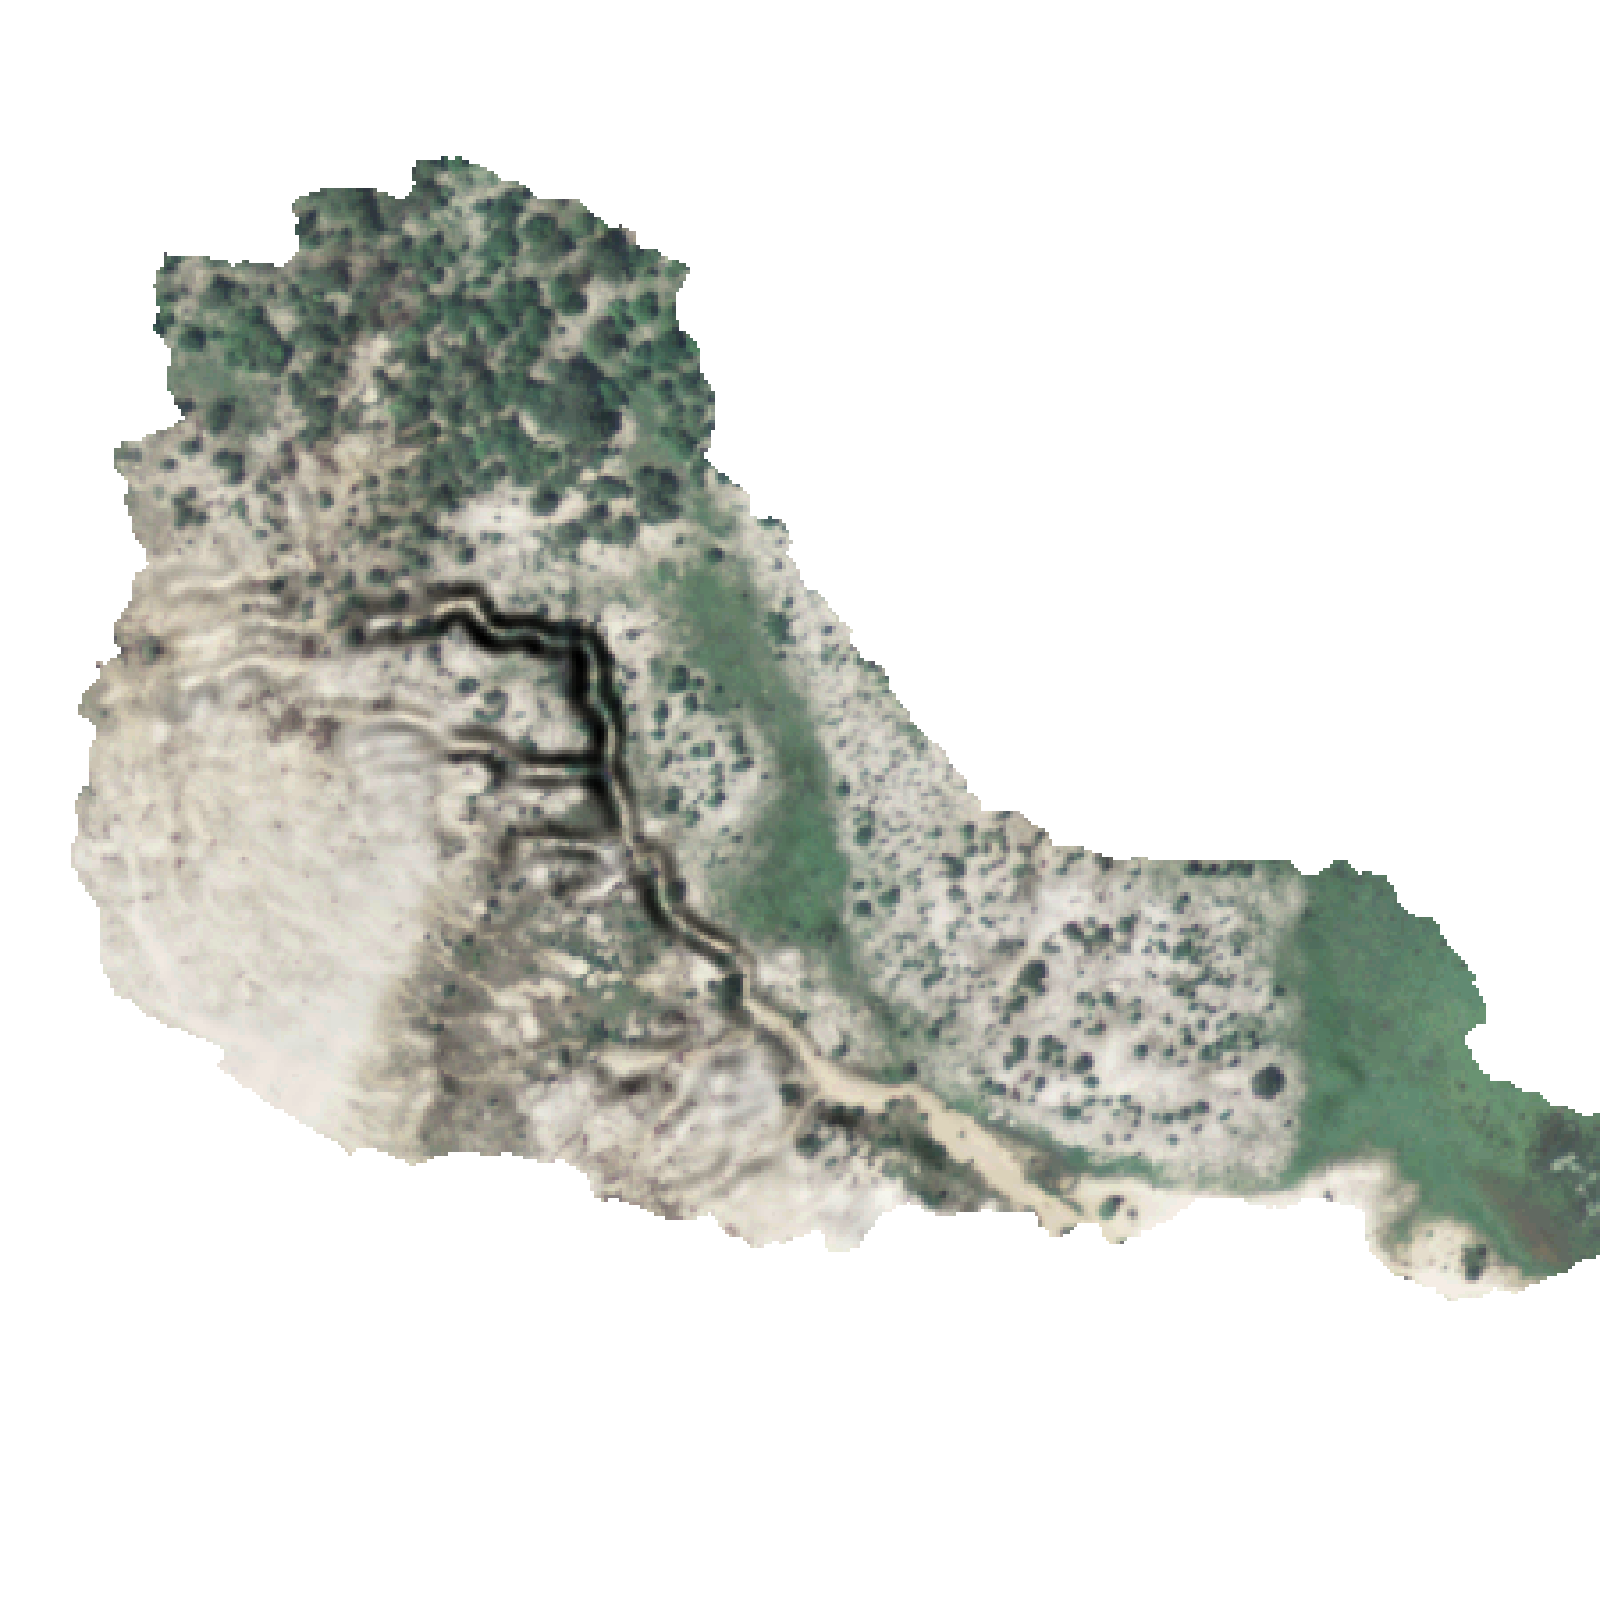
\includegraphics[height=50mm]{../images/sample_data/naip_2014.png}} &
\multicolumn{1}{c}{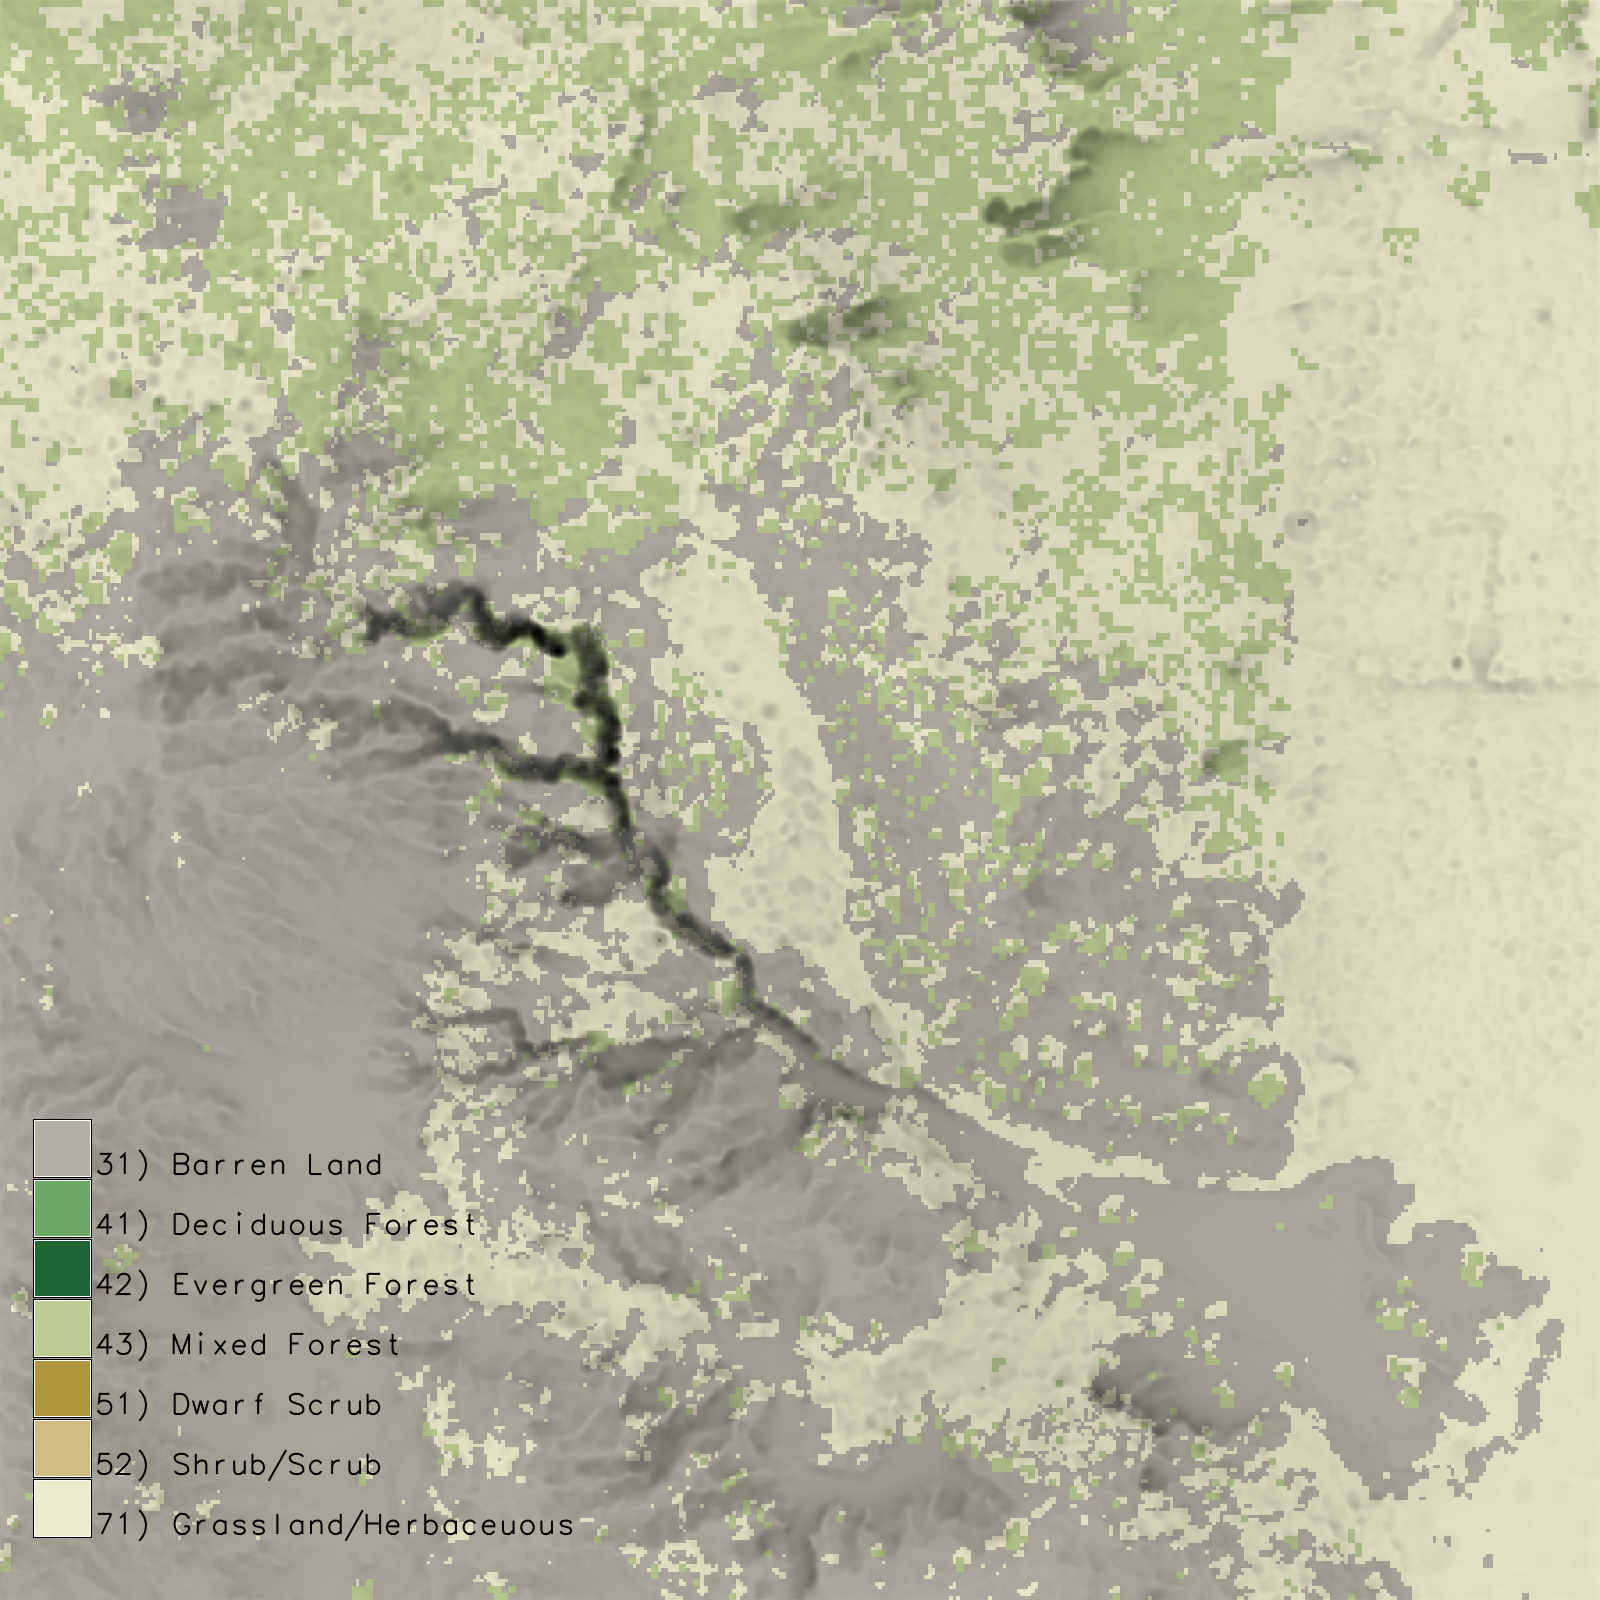
\includegraphics[height=50mm]{../images/sample_data/landcover.png}}\\
\multicolumn{1}{c}{Orthophotograph} & \multicolumn{1}{c}{Landcover}\\
%
\multicolumn{1}{c}{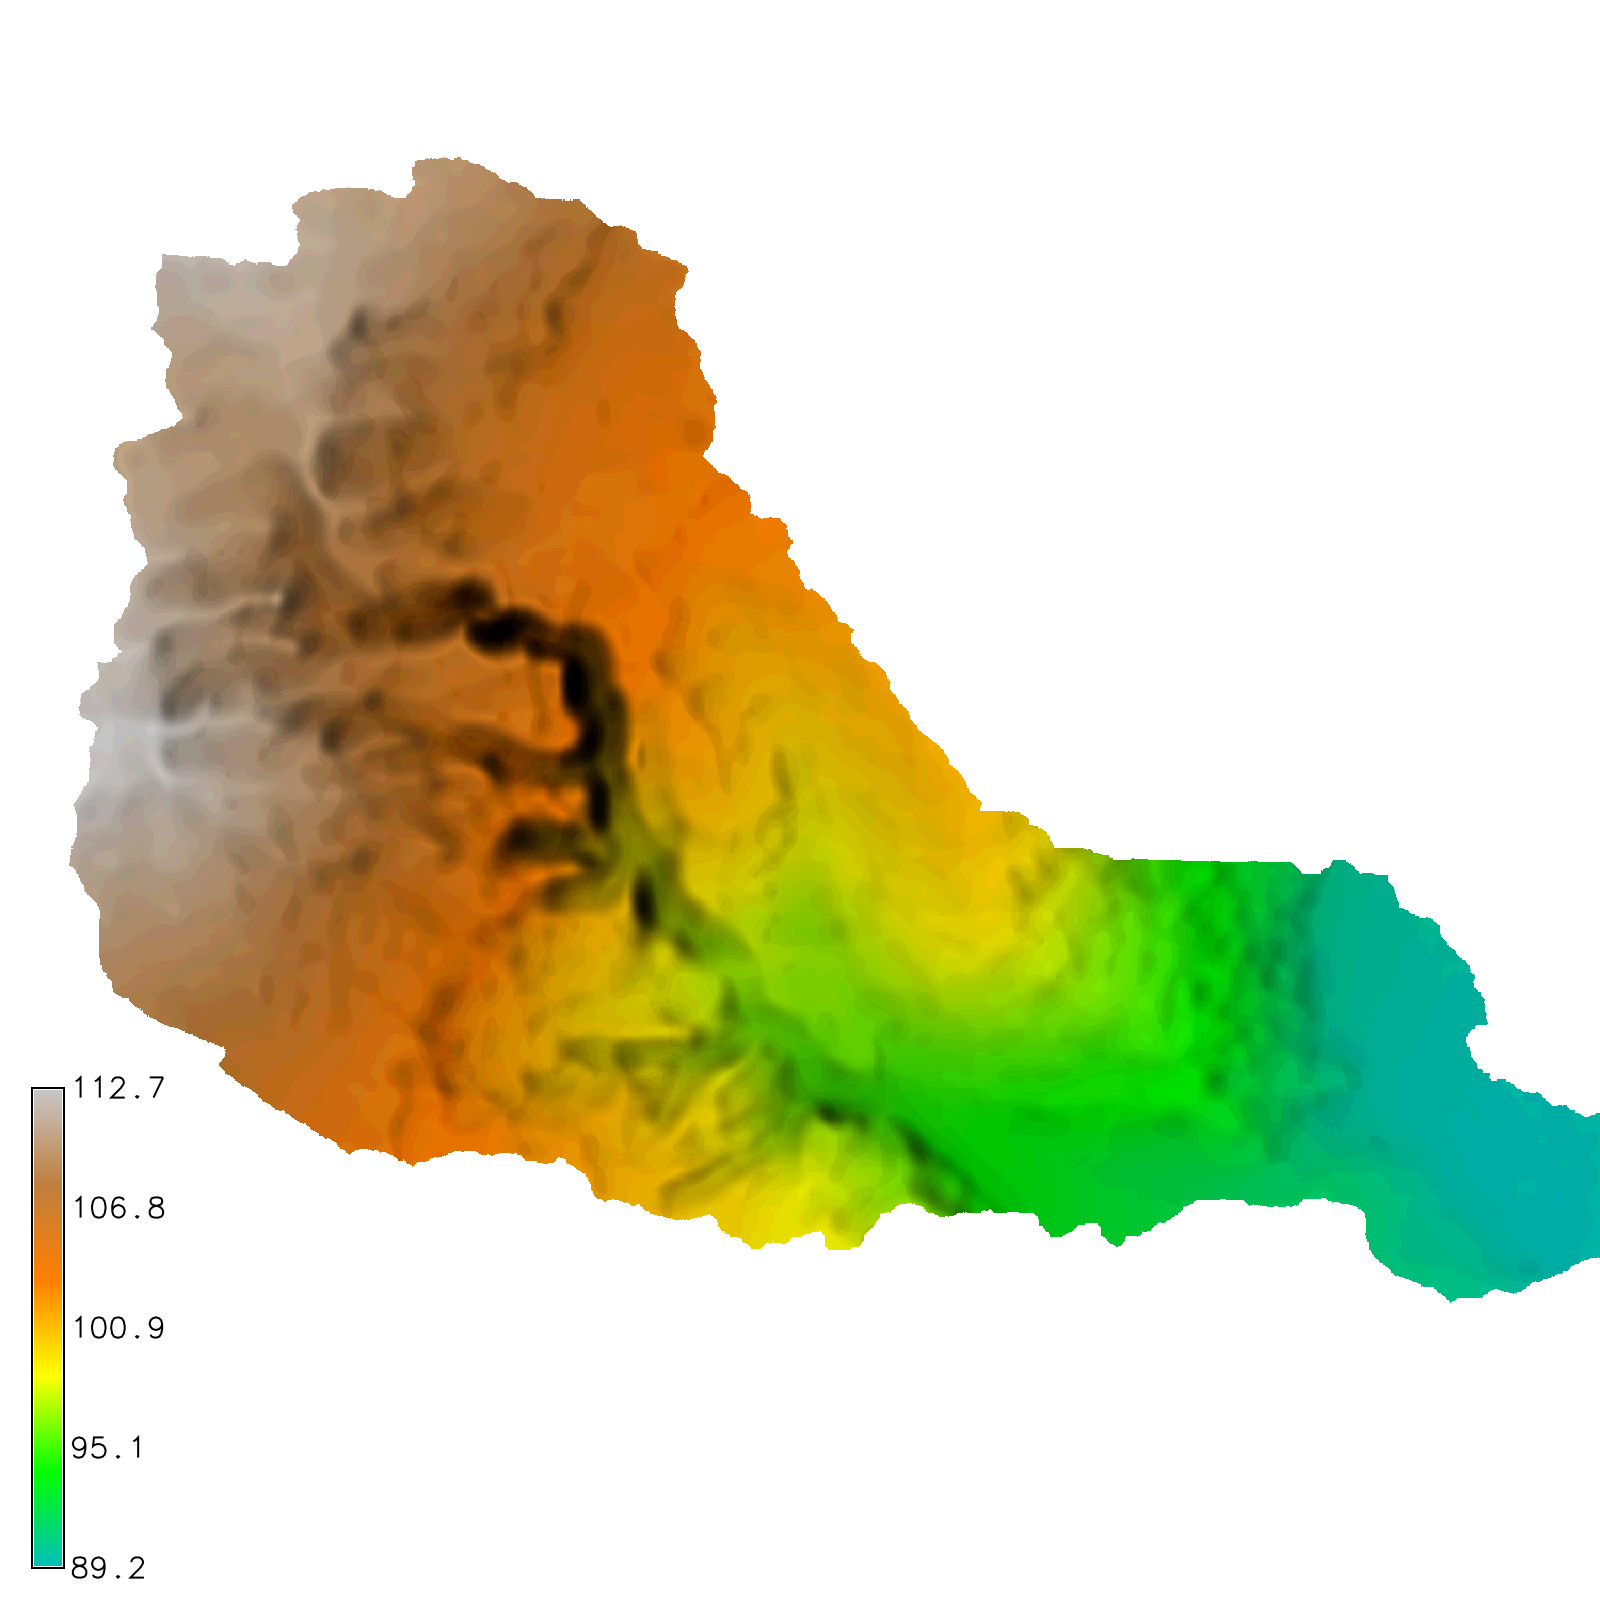
\includegraphics[height=50mm]{../images/sample_data/elevation_2004.png}} &
\multicolumn{1}{c}{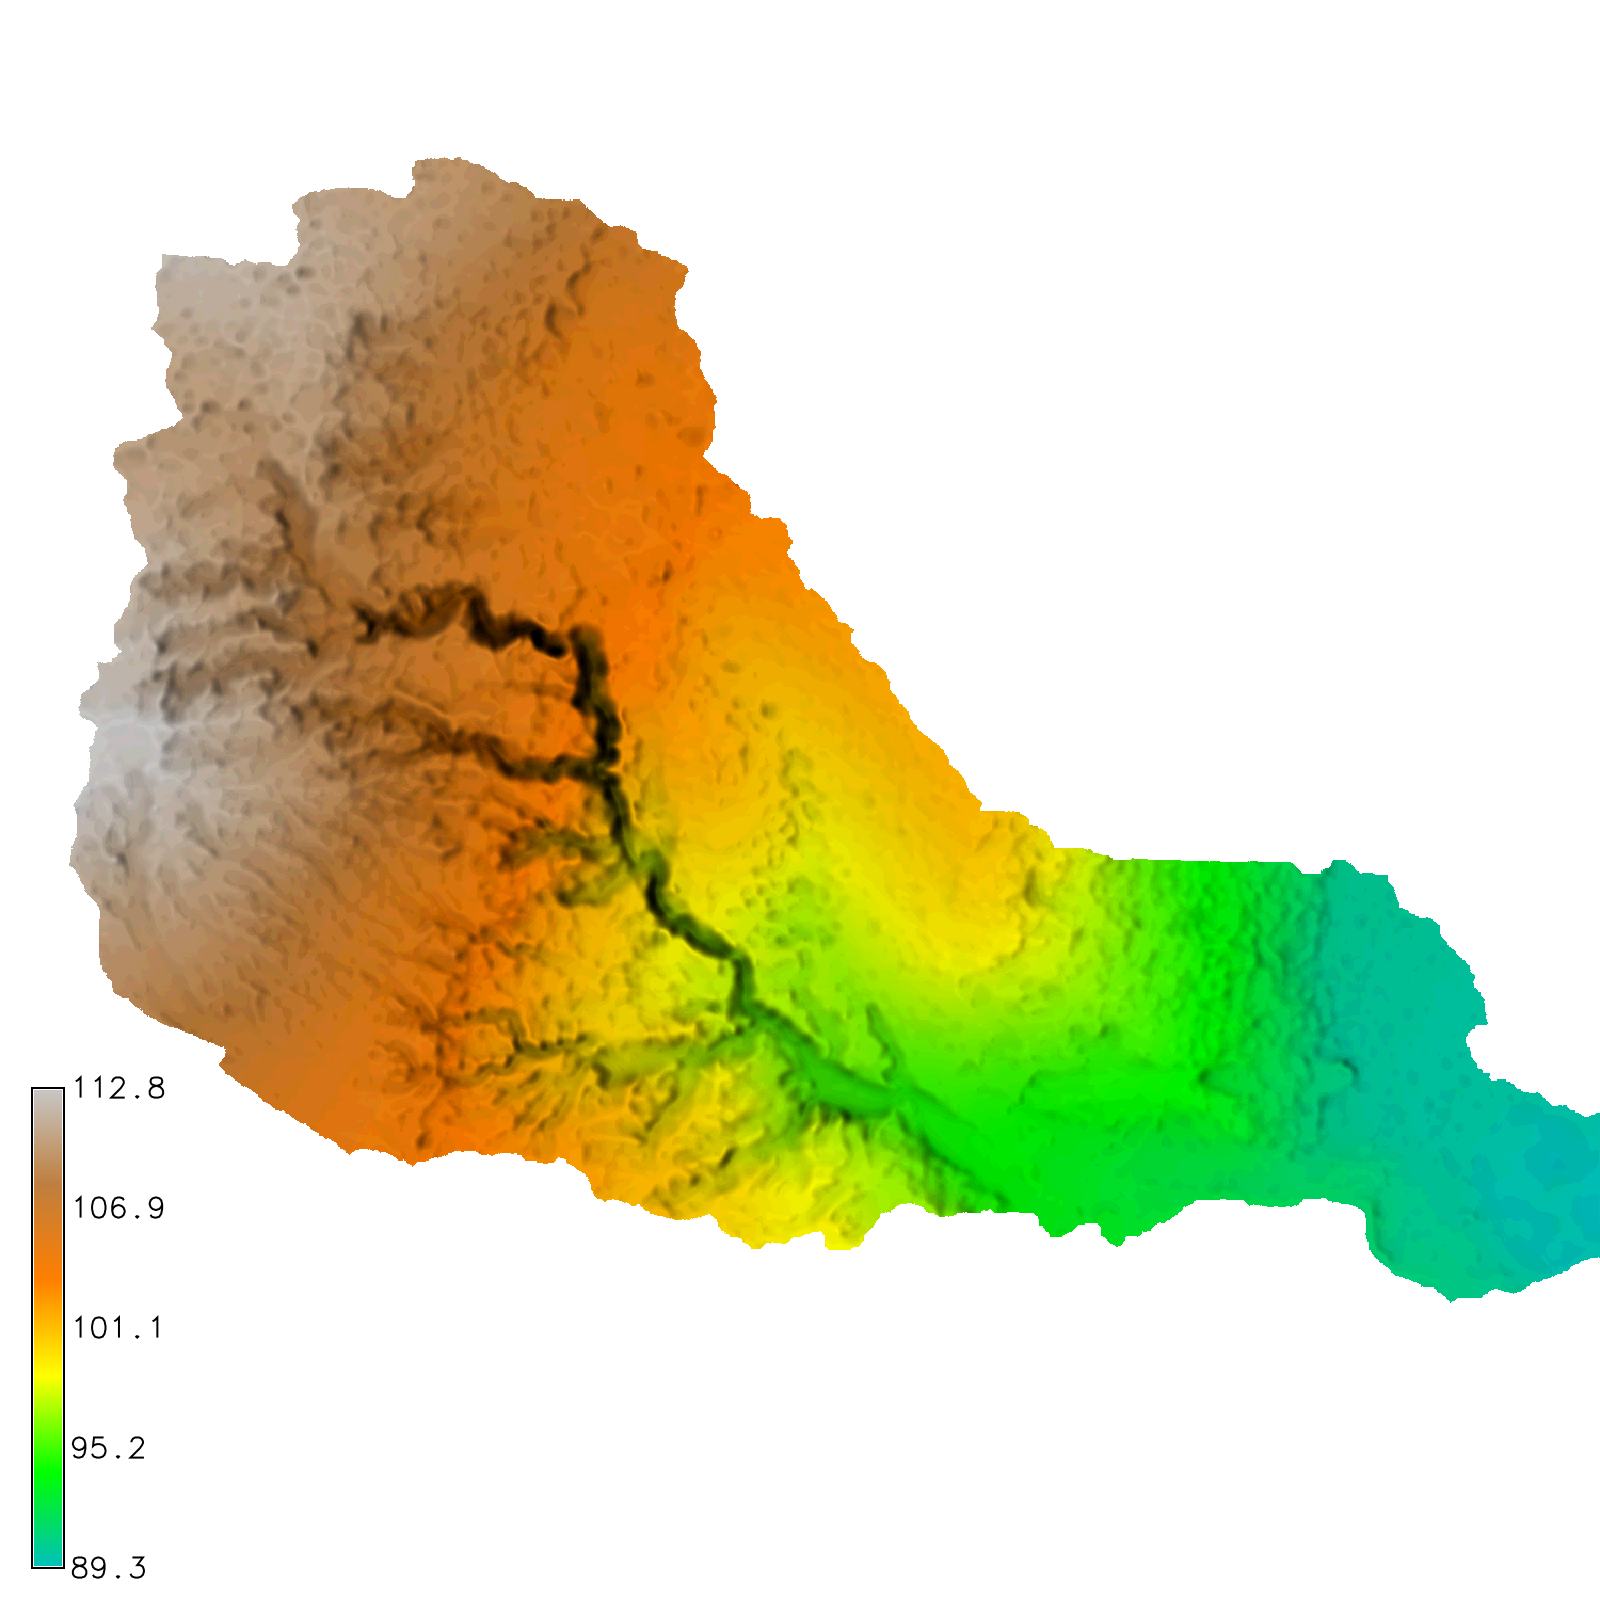
\includegraphics[height=50mm]{../images/sample_data/elevation_2016.png}}\\
\multicolumn{1}{c}{Elevation 2004} & \multicolumn{1}{c}{Elevation 2016}\\
%
\multicolumn{1}{c}{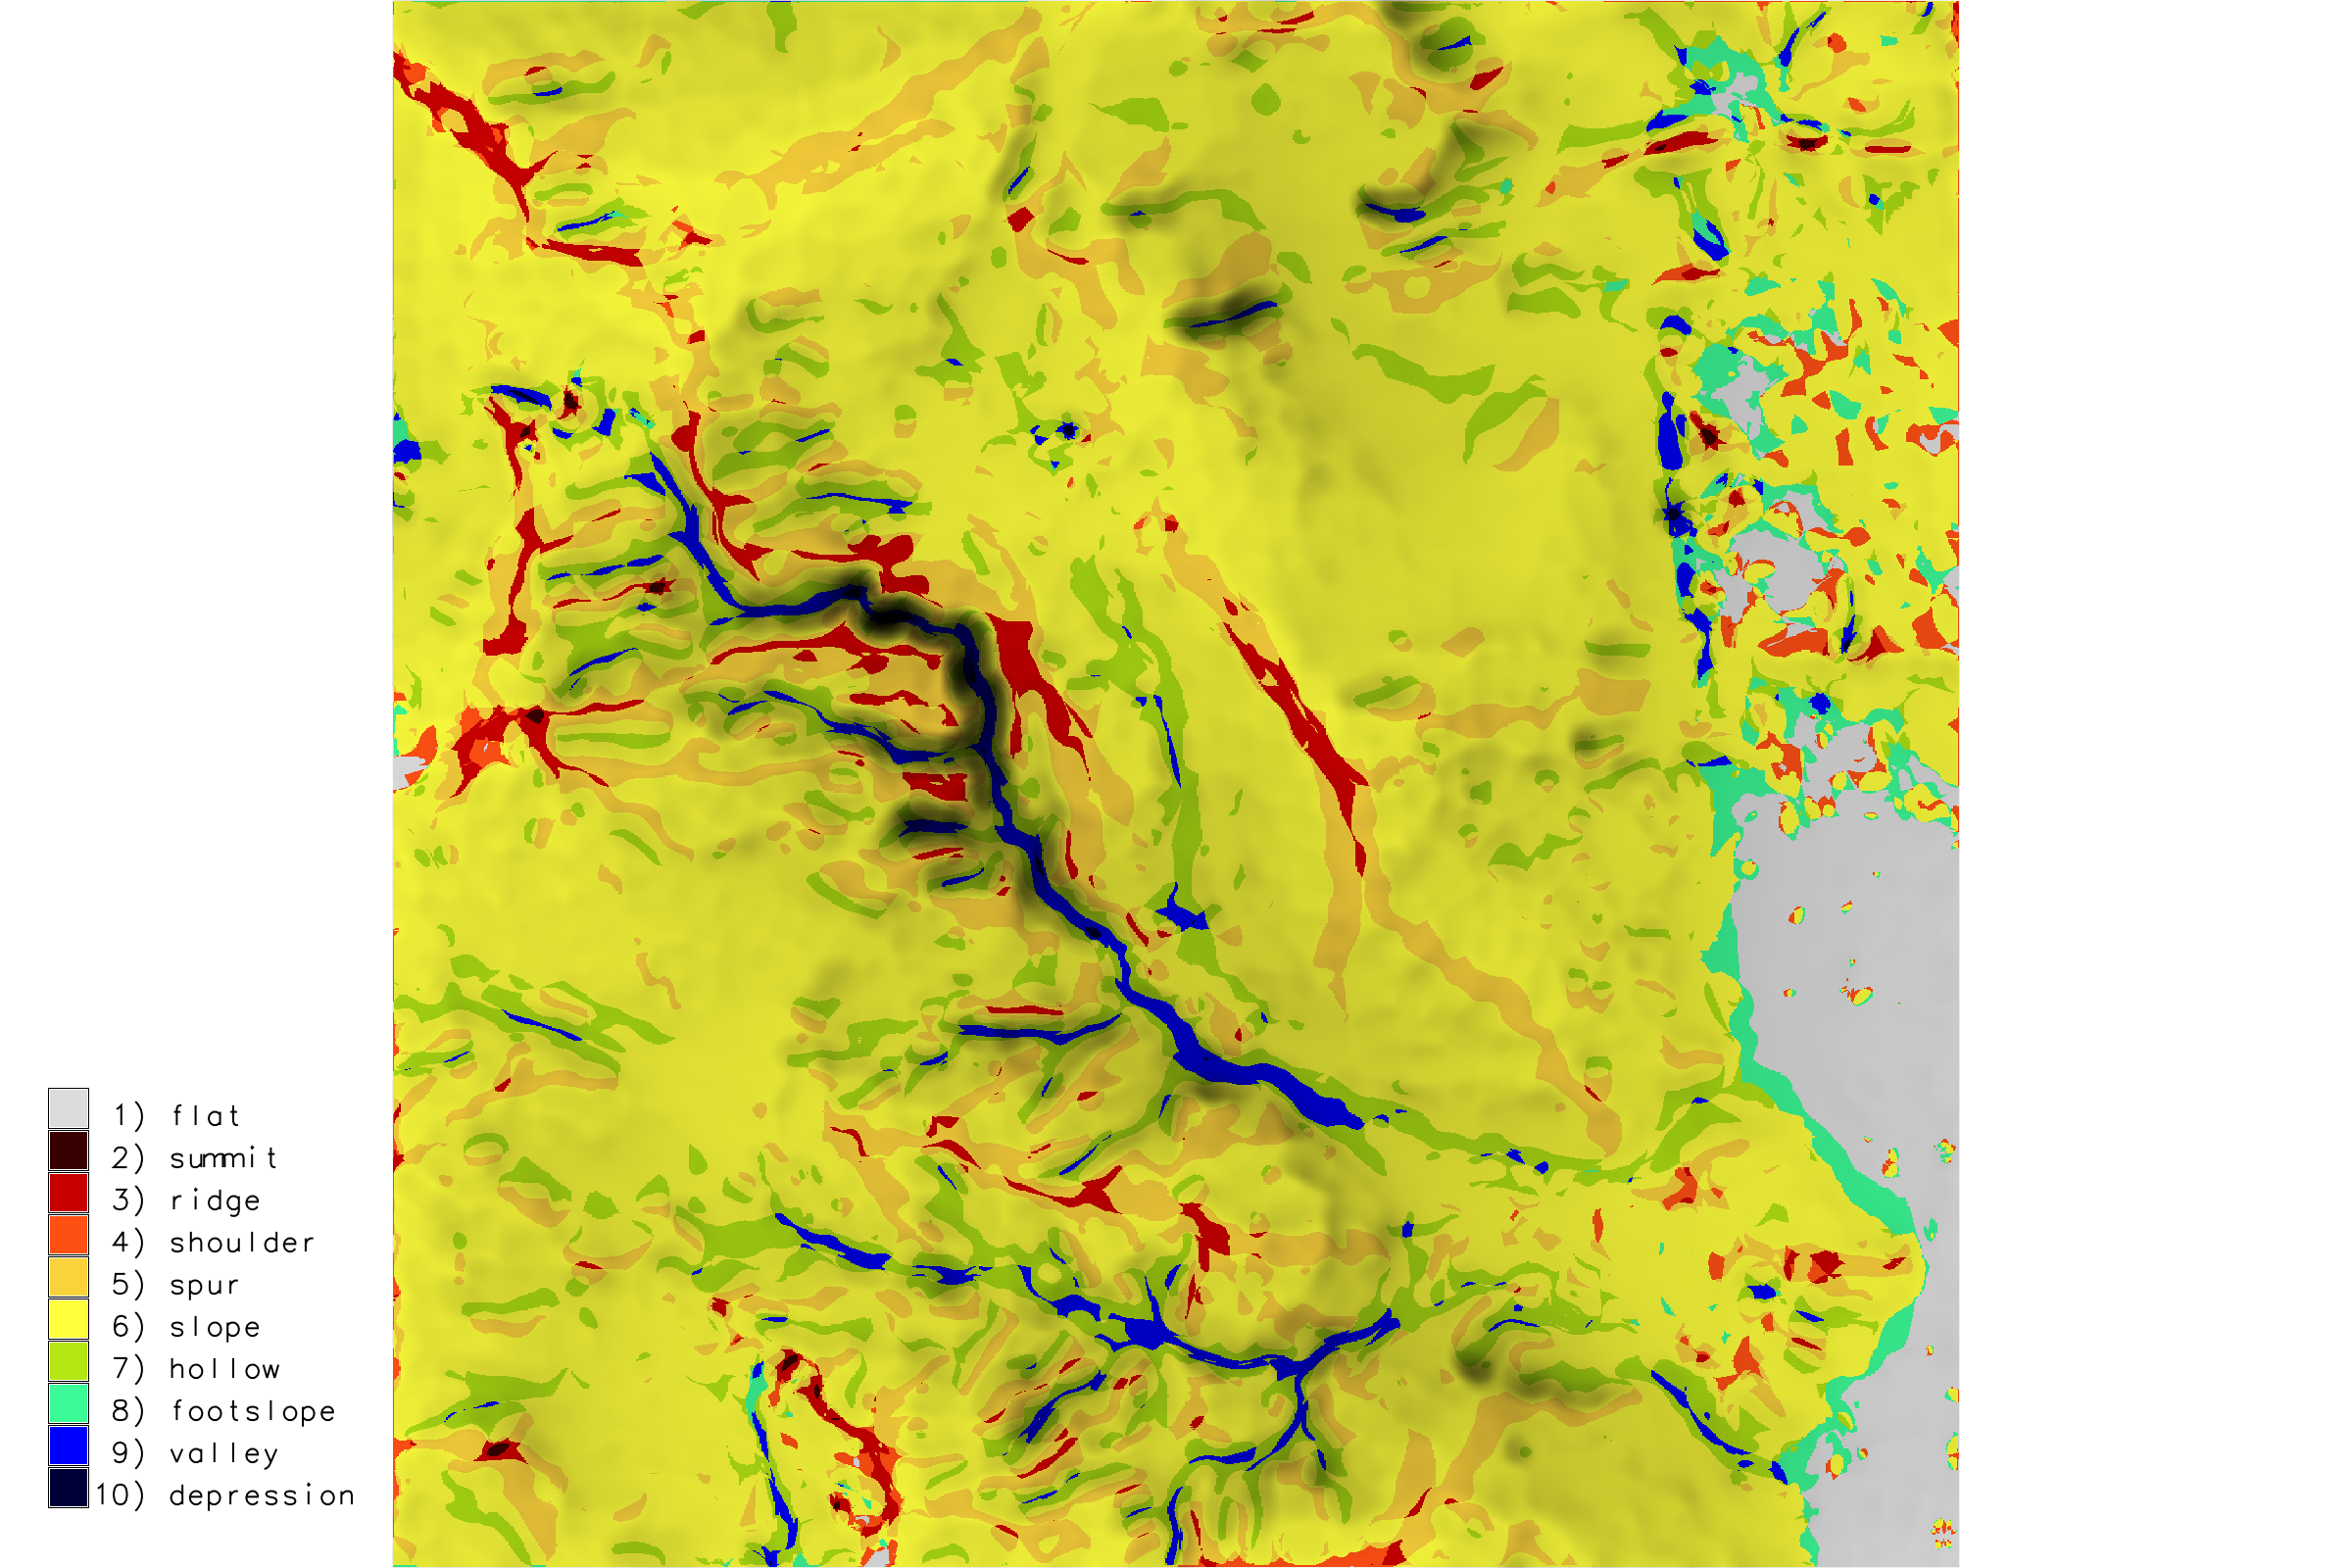
\includegraphics[height=50mm]{../images/sample_data/landforms_2004.png}} &
\multicolumn{1}{c}{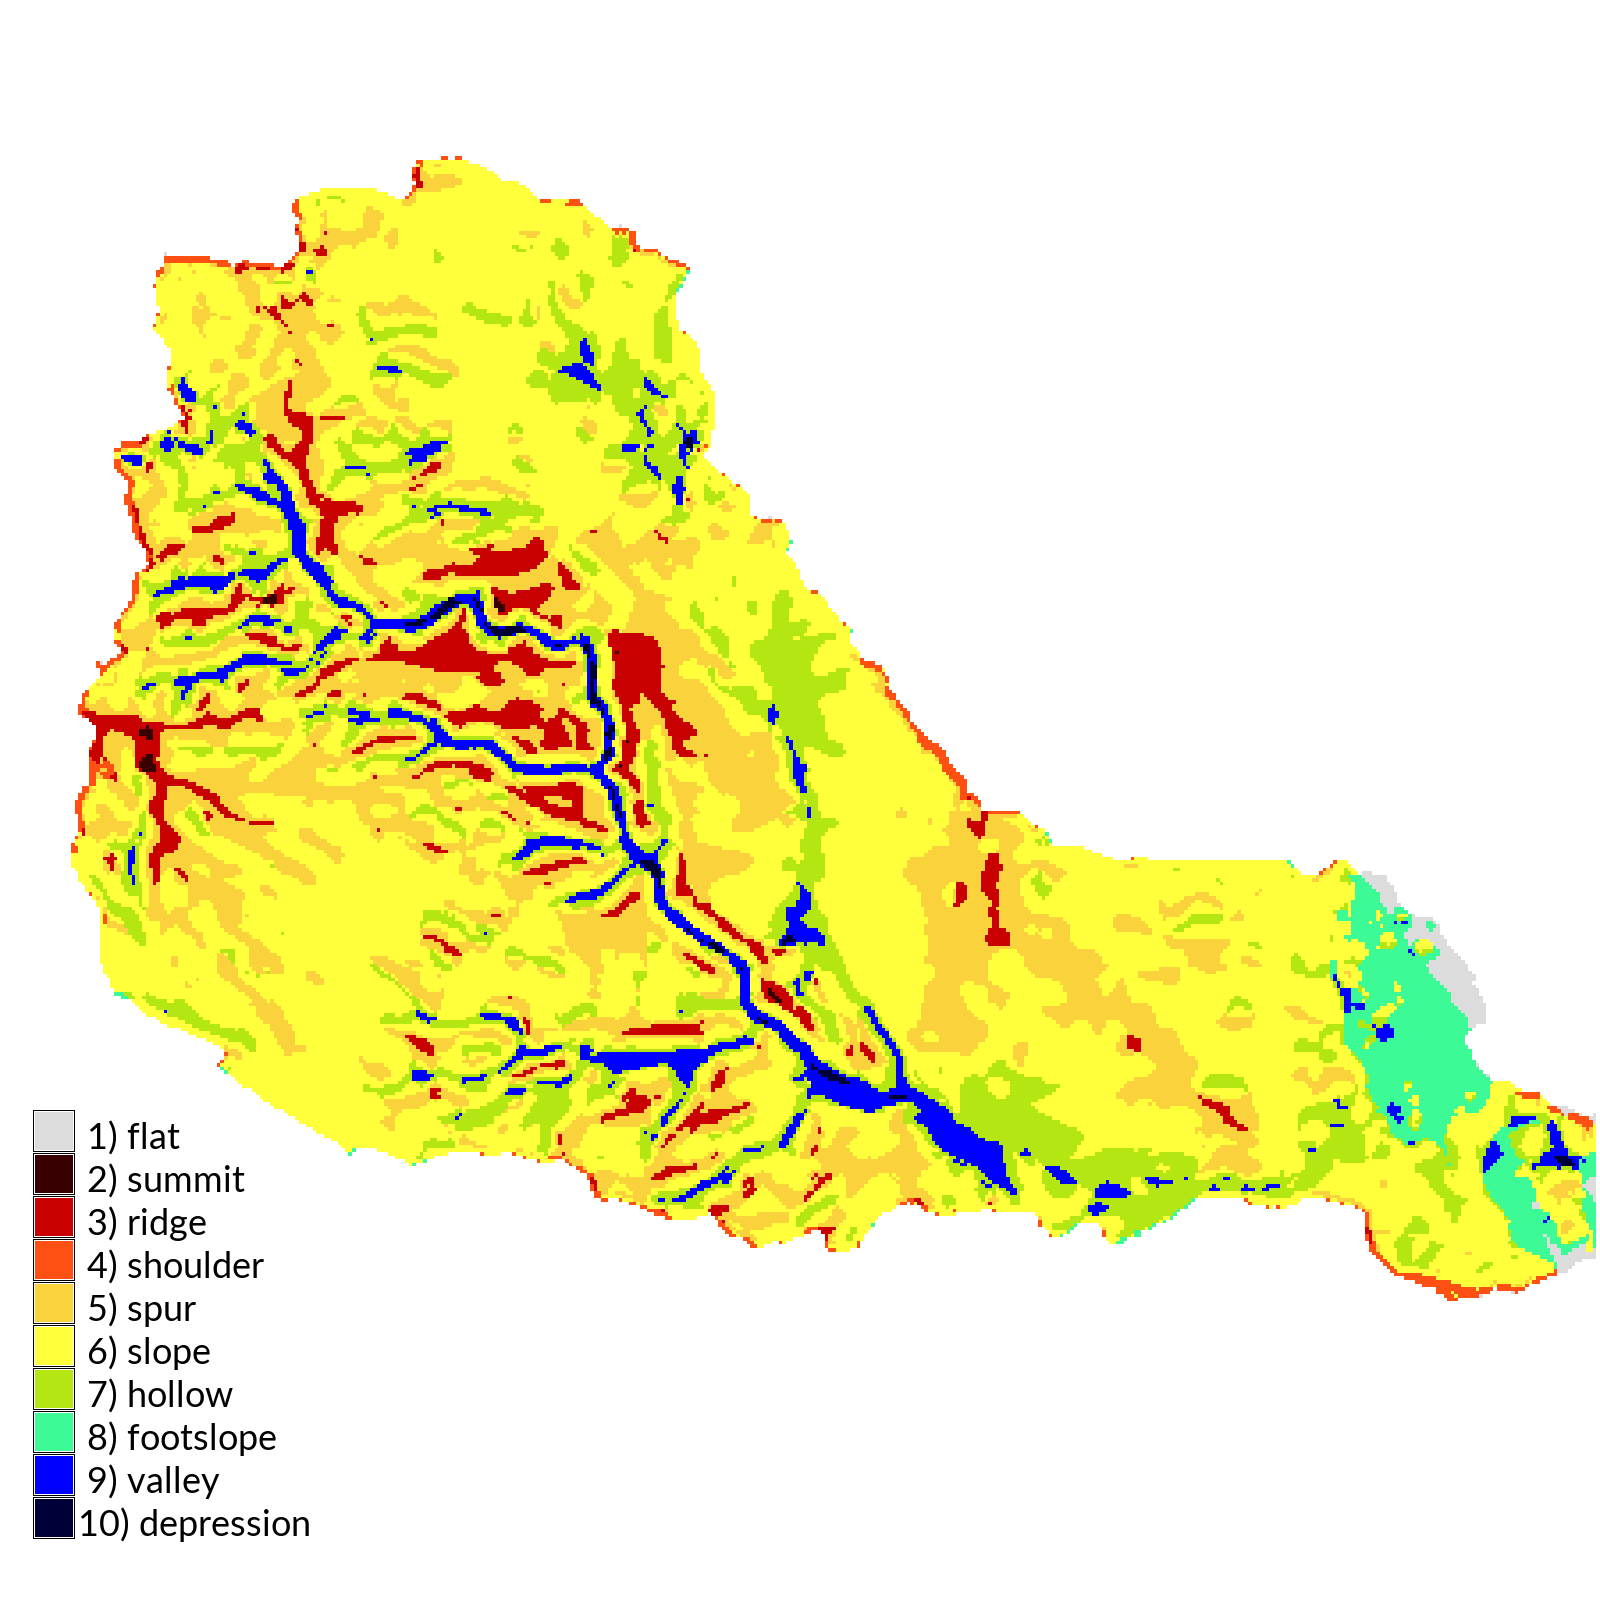
\includegraphics[height=50mm]{../images/sample_data/landforms_2016.png}}\\
\multicolumn{1}{c}{Landforms 2004} & \multicolumn{1}{c}{Landforms 2016}\\
%
\multicolumn{1}{c}{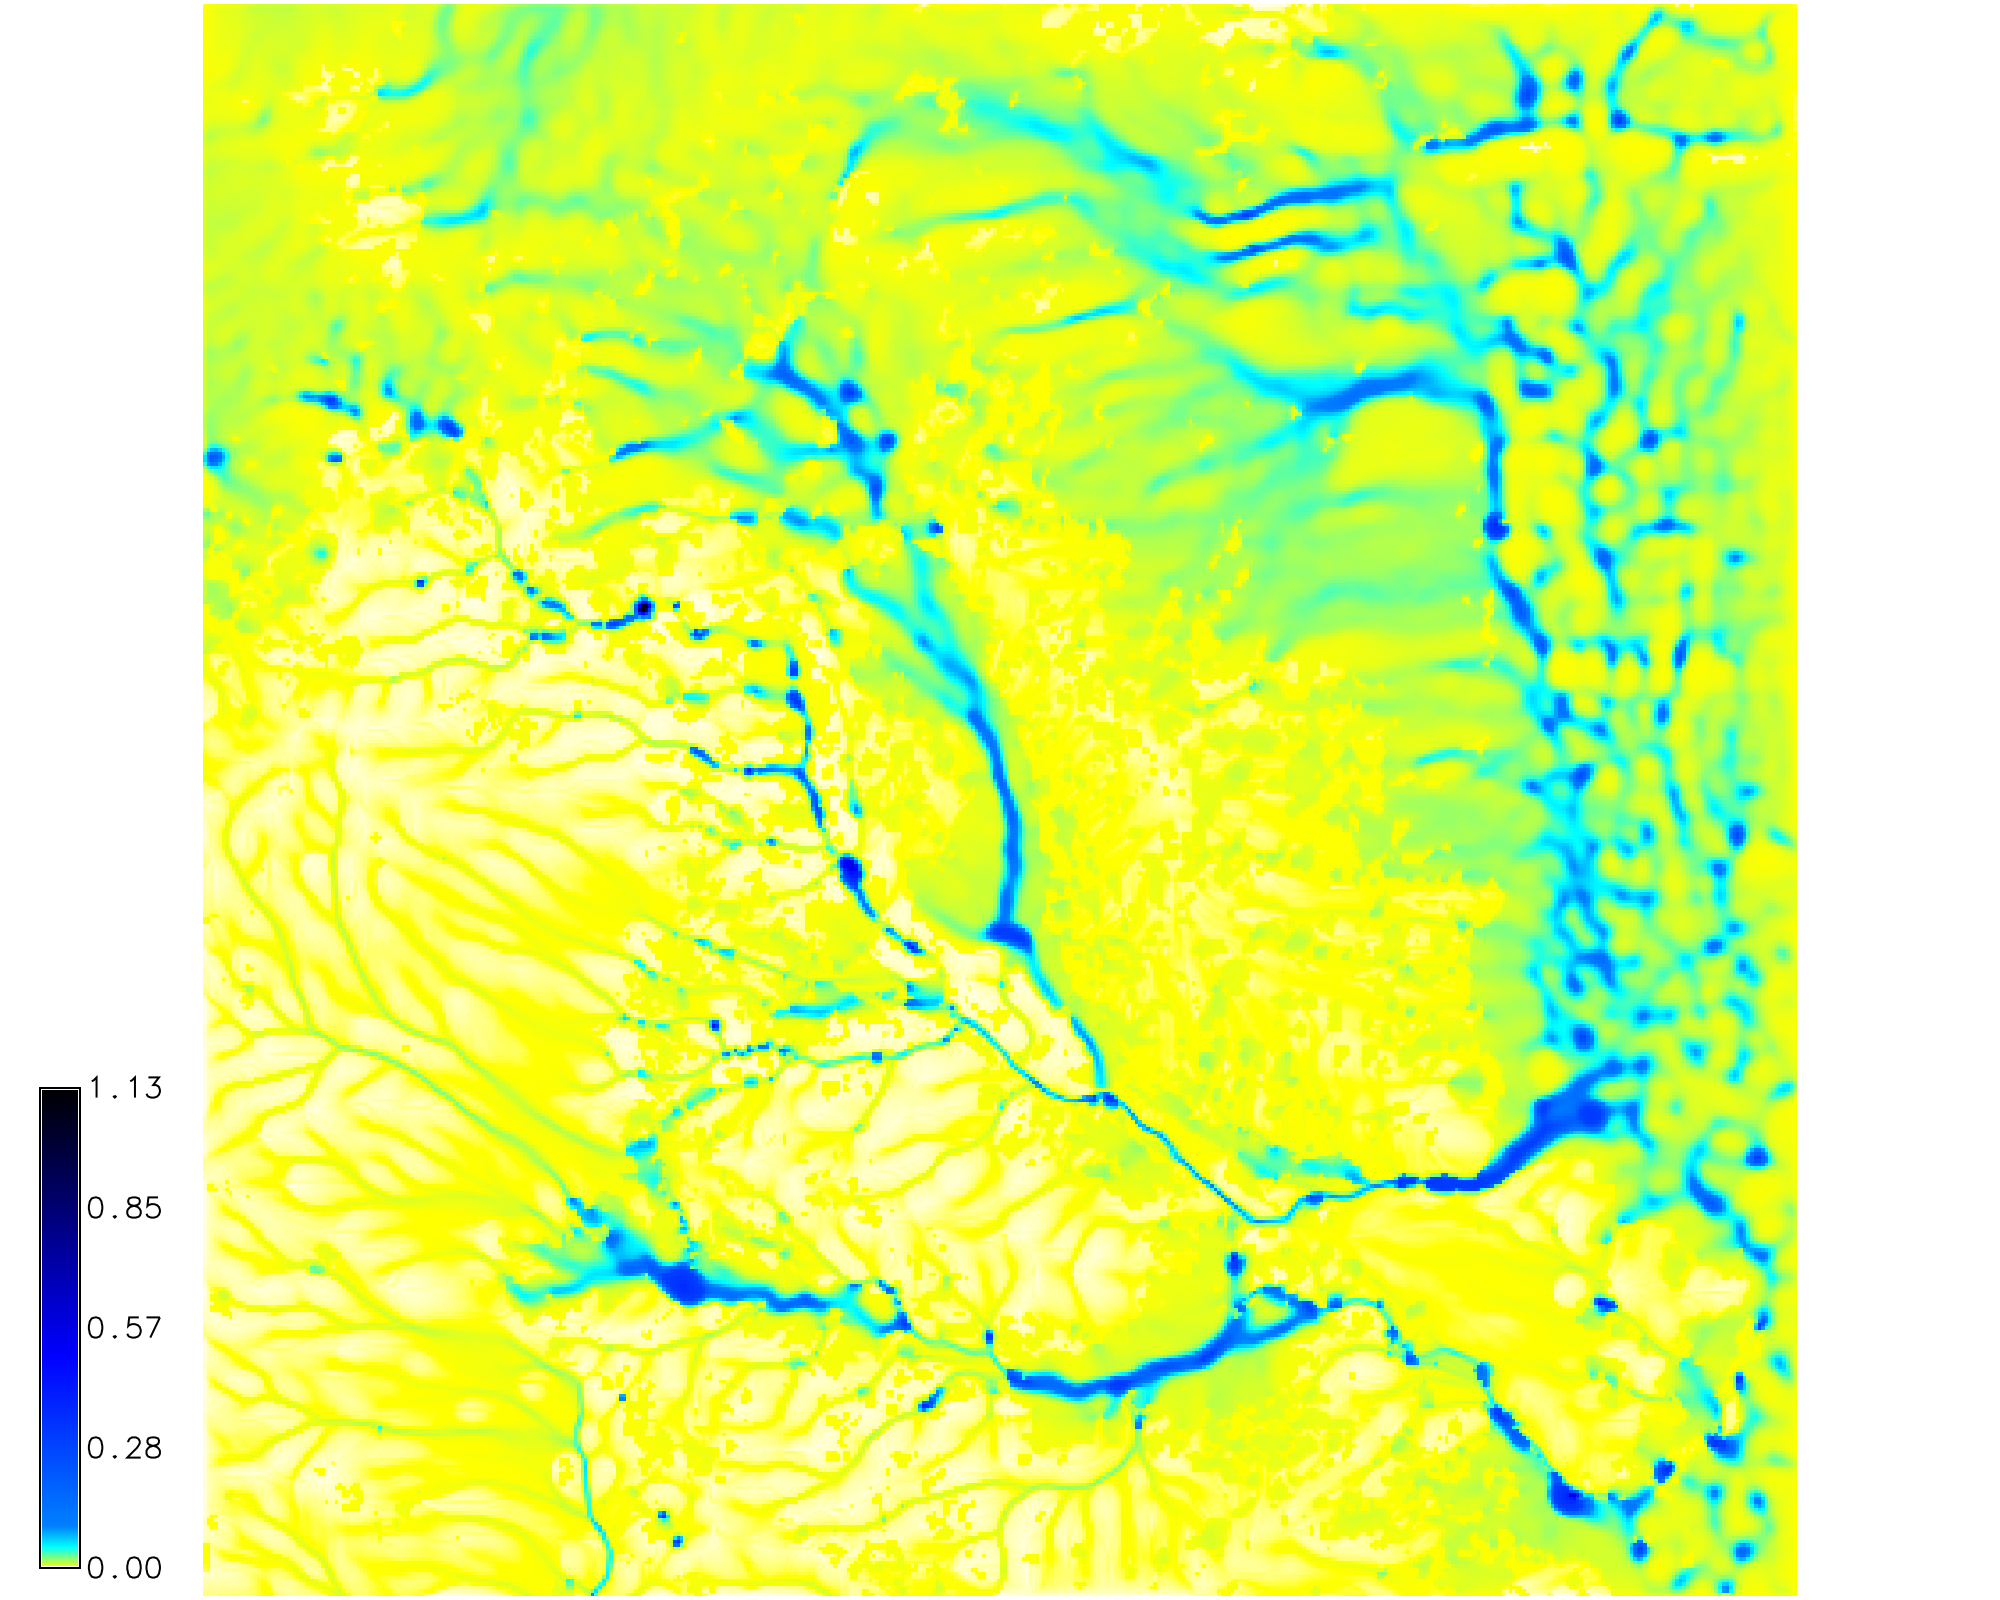
\includegraphics[height=50mm]{../images/sample_data/depth_2016.png}} &
\multicolumn{1}{c}{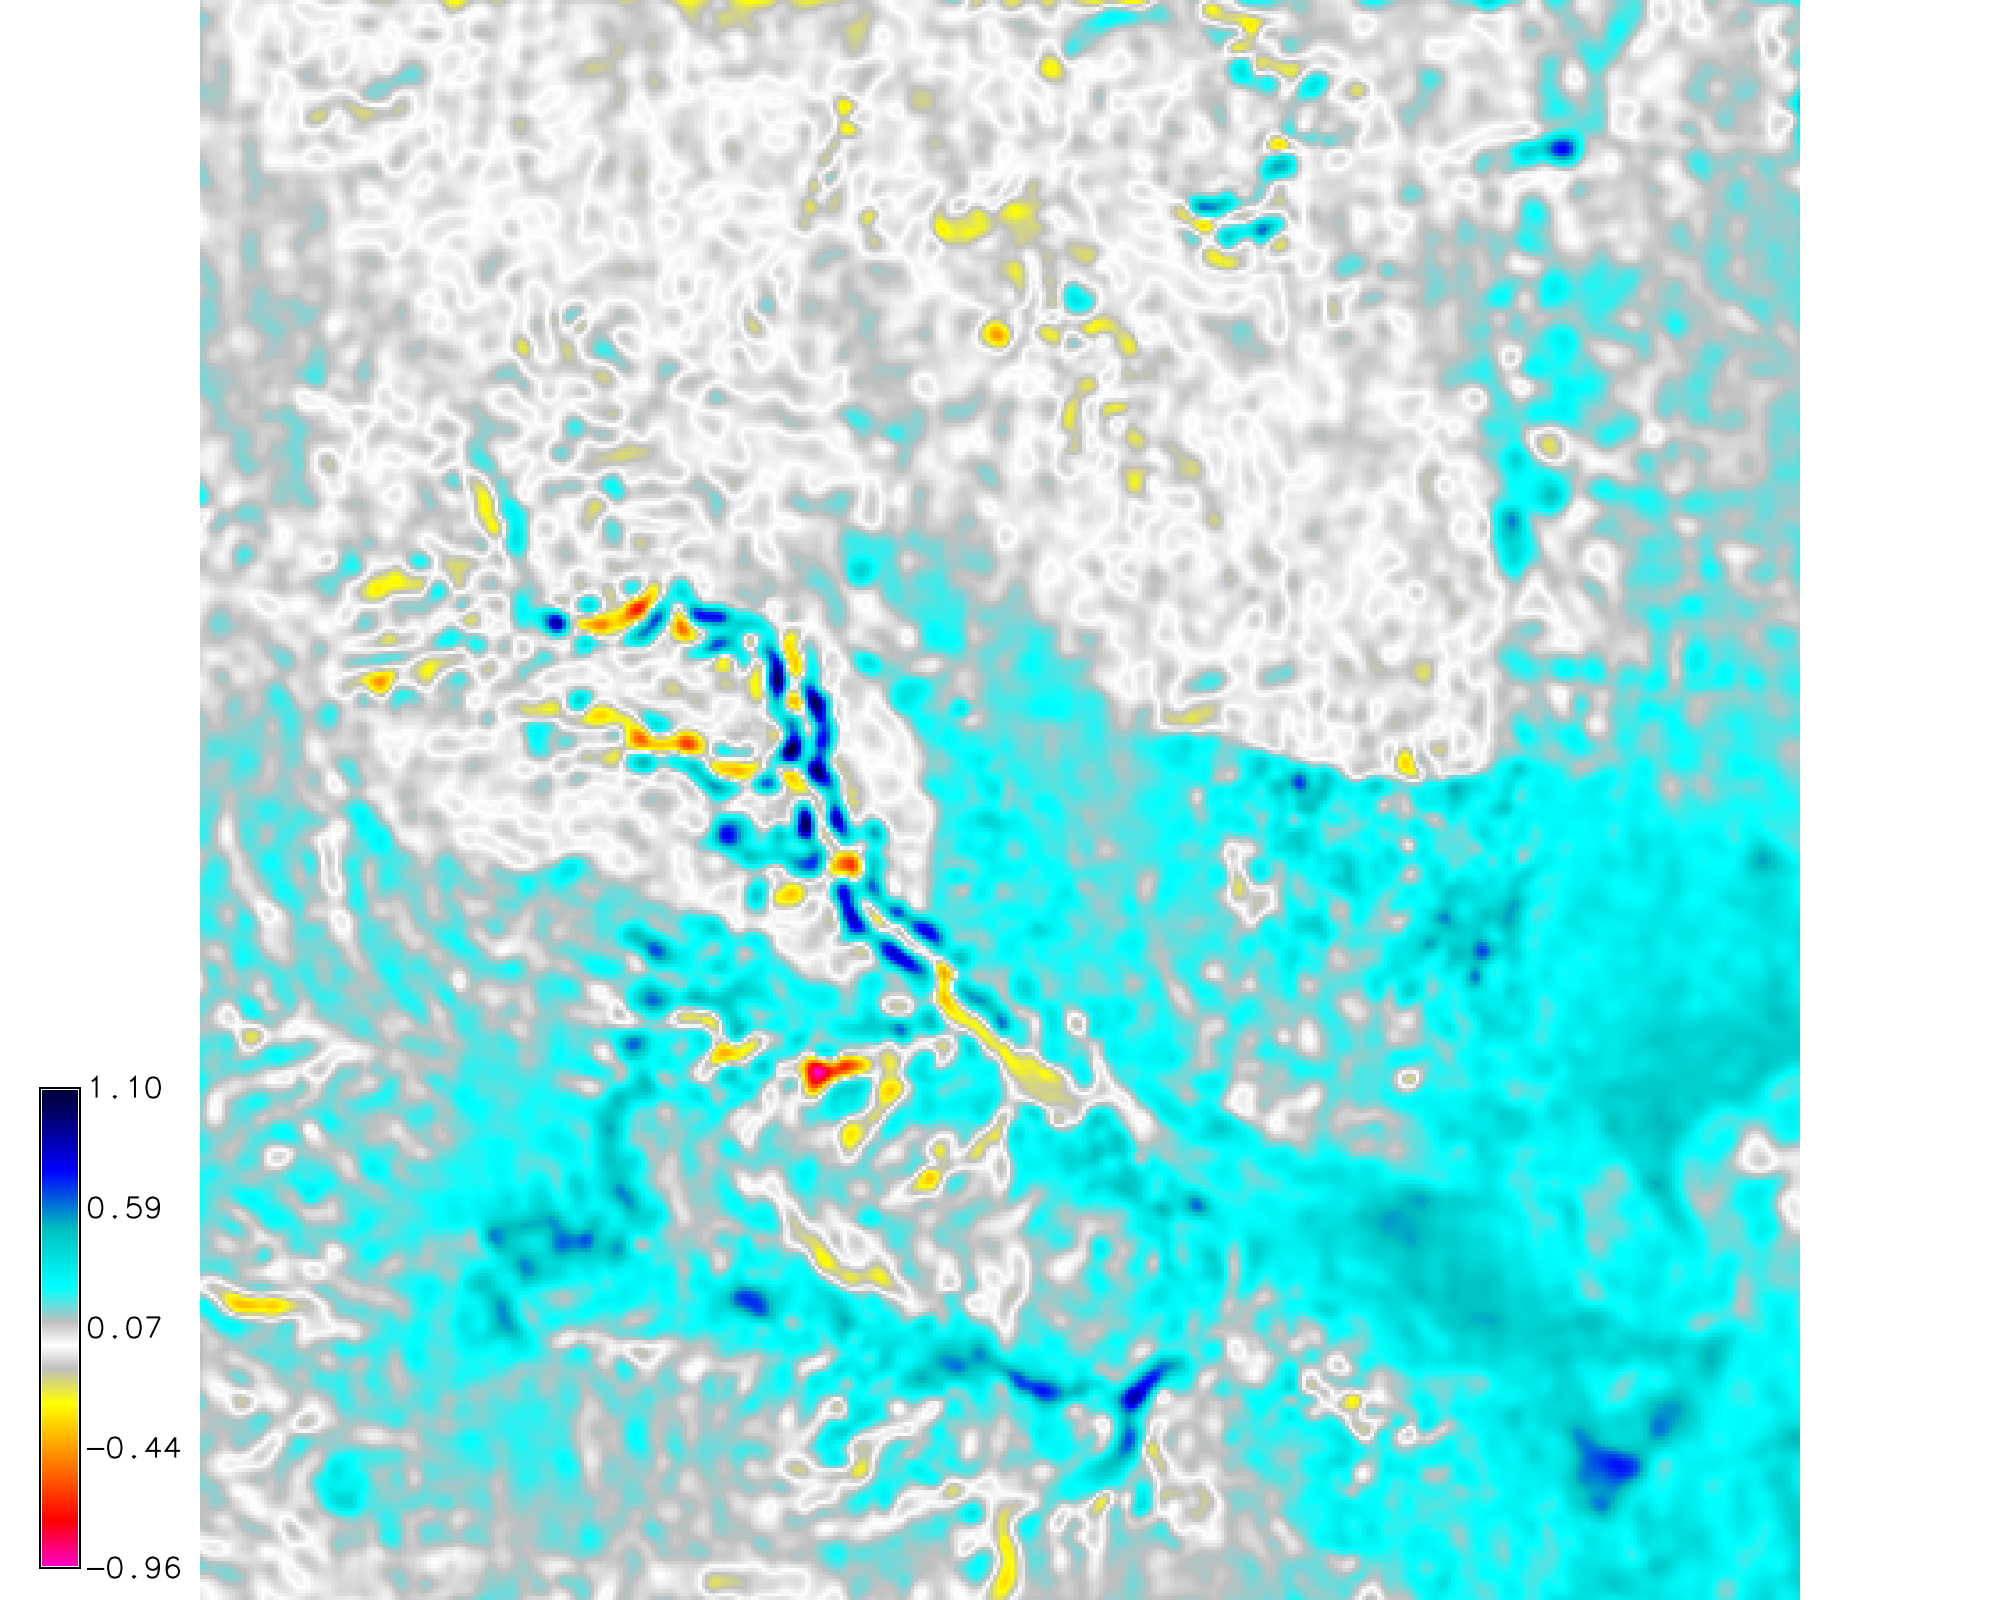
\includegraphics[height=50mm]{../images/sample_data/difference_2004_2016.png}}\\
\multicolumn{1}{c}{Water depth for 10 min event with 50mm/hr} & \multicolumn{1}{c}{Difference 2004-2016}\\
%
\end{tabular}
\caption{Study Landscape, Patterson Branch Creek, Fort Bragg, NC, USA}
\label{fig:study_area}
%
\end{figure*}